\documentclass{standalone}
\usepackage{tikz}
\usetikzlibrary{patterns, positioning}
\usepackage[sfdefault]{ClearSans} %% option 'sfdefault' activates Clear Sans as the default text font
\usepackage[T1]{fontenc}

\begin{document}
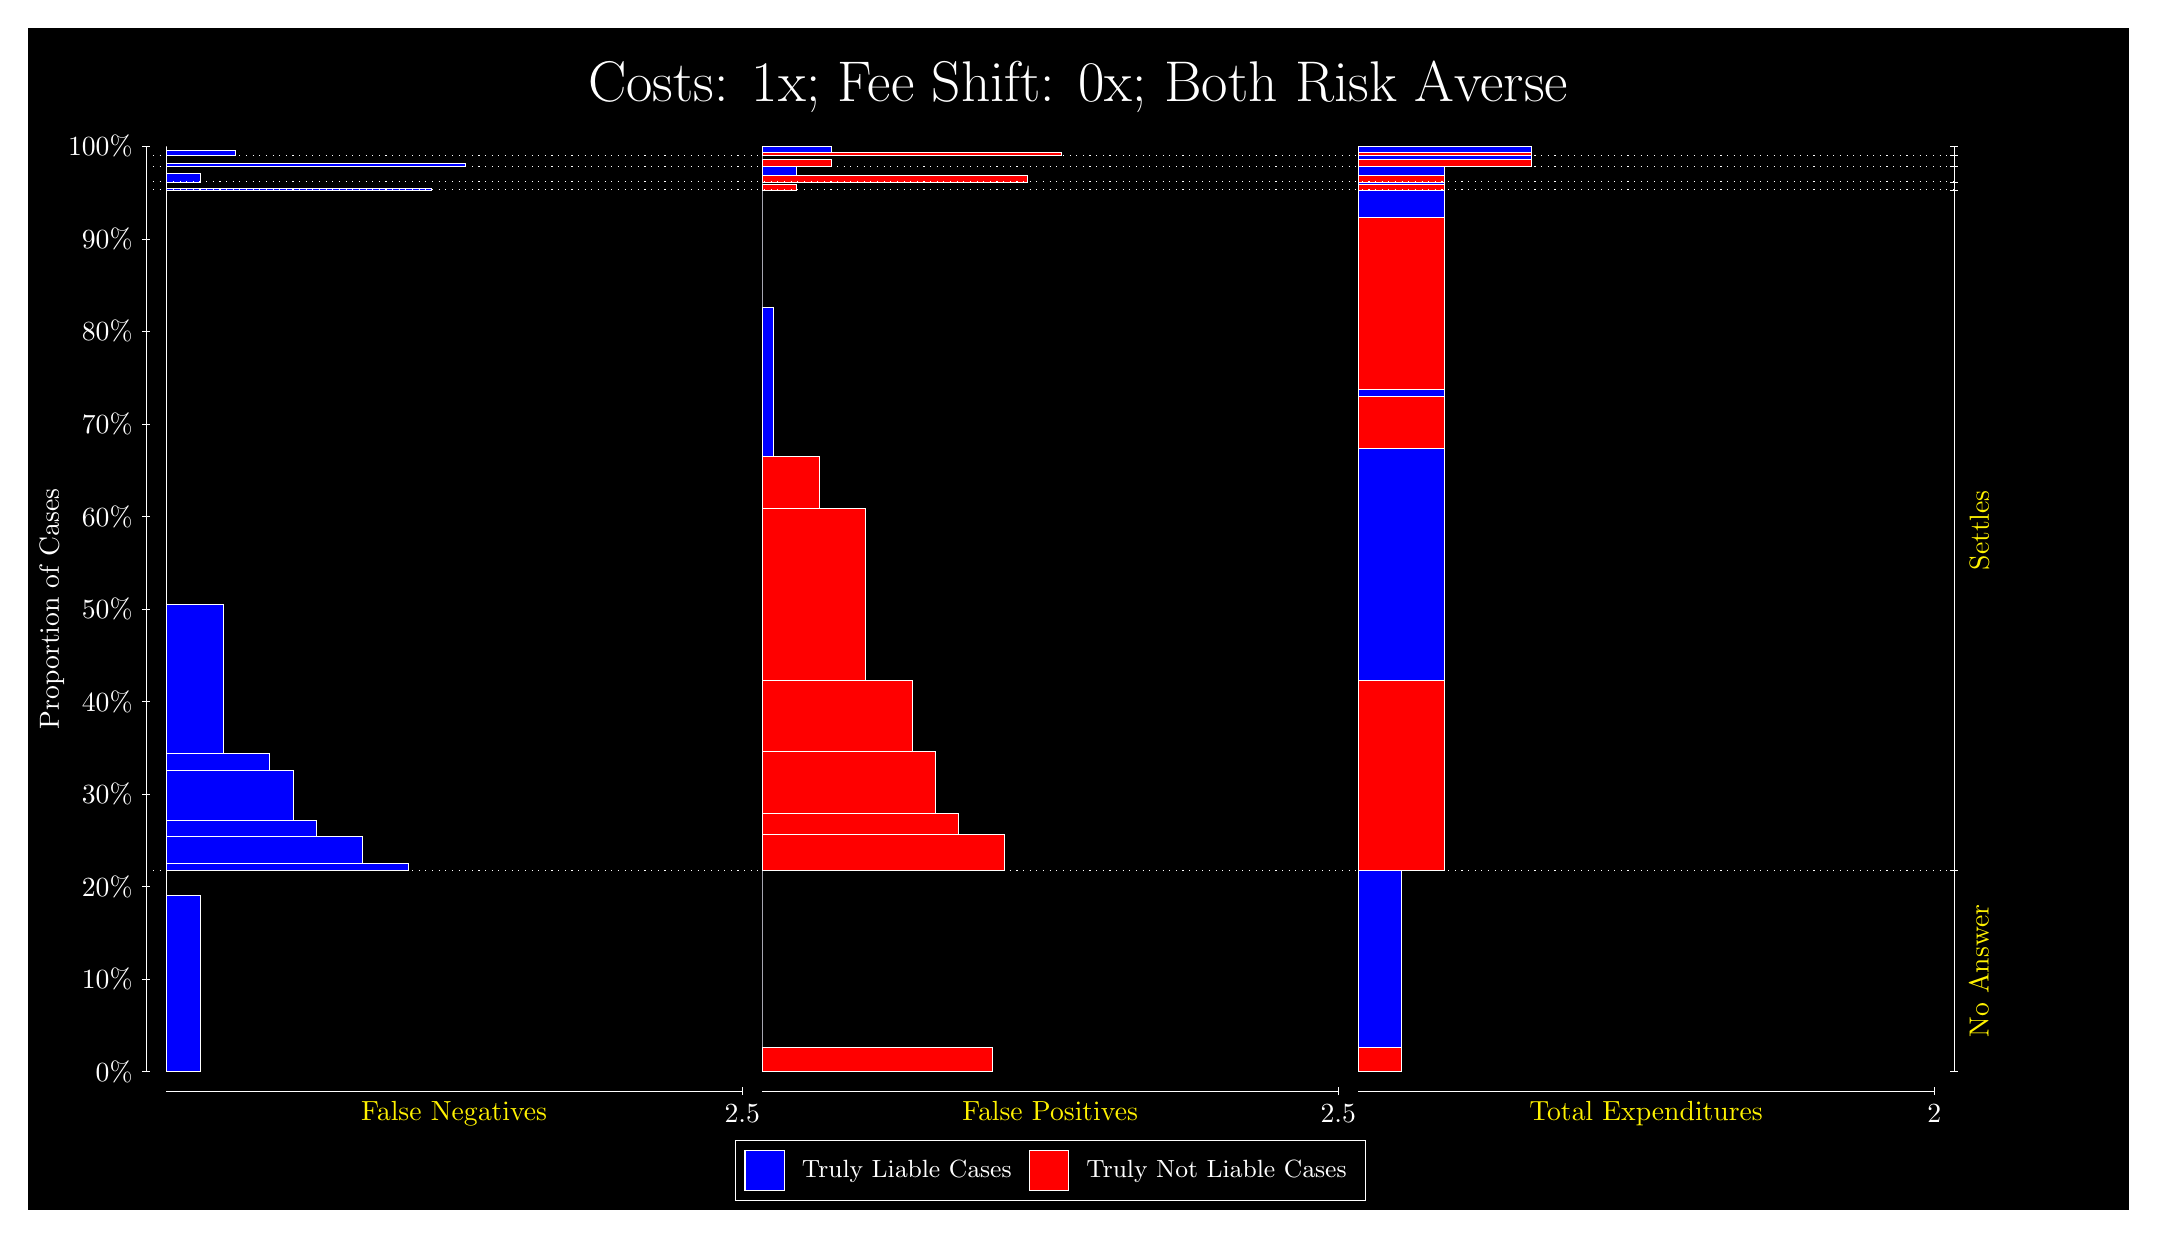
\begin{tikzpicture}
\draw[fill=black] (0,0) rectangle (26.667,15);
\draw[text=white] (0,13.5) rectangle (26.667,15) node[midway] {\huge Costs: 1x; Fee Shift: 0x; Both Risk Averse};
\draw[white, very thin] (1.5,1.75) -- (1.5,13.5);
\node[rotate=90, text=white, anchor=center] at (0.3, 7.625) {Proportion of Cases};
\draw[white, very thin] (1.45,1.75) -- (1.55,1.75);
\node[text=white, anchor=east] at (1.45, 1.75) {0\%};
\draw[white, very thin] (1.45,2.925) -- (1.55,2.925);
\node[text=white, anchor=east] at (1.45, 2.925) {10\%};
\draw[white, very thin] (1.45,4.1) -- (1.55,4.1);
\node[text=white, anchor=east] at (1.45, 4.1) {20\%};
\draw[white, very thin] (1.45,5.275) -- (1.55,5.275);
\node[text=white, anchor=east] at (1.45, 5.275) {30\%};
\draw[white, very thin] (1.45,6.45) -- (1.55,6.45);
\node[text=white, anchor=east] at (1.45, 6.45) {40\%};
\draw[white, very thin] (1.45,7.625) -- (1.55,7.625);
\node[text=white, anchor=east] at (1.45, 7.625) {50\%};
\draw[white, very thin] (1.45,8.8) -- (1.55,8.8);
\node[text=white, anchor=east] at (1.45, 8.8) {60\%};
\draw[white, very thin] (1.45,9.975) -- (1.55,9.975);
\node[text=white, anchor=east] at (1.45, 9.975) {70\%};
\draw[white, very thin] (1.45,11.15) -- (1.55,11.15);
\node[text=white, anchor=east] at (1.45, 11.15) {80\%};
\draw[white, very thin] (1.45,12.325) -- (1.55,12.325);
\node[text=white, anchor=east] at (1.45, 12.325) {90\%};
\draw[white, very thin] (1.45,13.5) -- (1.55,13.5);
\node[text=white, anchor=east] at (1.45, 13.5) {100\%};

\draw[white, very thin] (24.457,1.75) -- (24.457,13.5);
\draw[white, very thin] (24.407,1.75) -- (24.507,1.75);
\node[anchor=west] at (24.407, 1.75) {};
\draw[white, very thin] (24.407,4.3013) -- (24.507,4.3013);
\node[anchor=west] at (24.407, 4.3013) {};
\draw[white, very thin] (24.407,12.946) -- (24.507,12.946);
\node[anchor=west] at (24.407, 12.946) {};
\draw[white, very thin] (24.407,13.048) -- (24.507,13.048);
\node[anchor=west] at (24.407, 13.048) {};
\draw[white, very thin] (24.407,13.241) -- (24.507,13.241);
\node[anchor=west] at (24.407, 13.241) {};
\draw[white, very thin] (24.407,13.382) -- (24.507,13.382);
\node[anchor=west] at (24.407, 13.382) {};
\draw[white, very thin] (24.407,13.5) -- (24.507,13.5);
\node[anchor=west] at (24.407, 13.5) {};

\draw[white, very thin, fill=blue] (1.75,1.75) rectangle (2.1891,3.9871);
\draw[white, very thin, fill=red] (1.75,3.9871) rectangle (1.75,4.3013);
\draw[white, very thin, fill=blue] (1.75,4.3013) rectangle (4.8239,4.3919);
\draw[white, very thin, fill=blue] (1.75,4.3919) rectangle (4.2384,4.7404);
\draw[white, very thin, fill=blue] (1.75,4.7404) rectangle (3.6529,4.9461);
\draw[white, very thin, fill=blue] (1.75,4.9461) rectangle (3.3602,5.582);
\draw[white, very thin, fill=blue] (1.75,5.582) rectangle (3.0674,5.7968);
\draw[white, very thin, fill=blue] (1.75,5.7968) rectangle (2.4819,7.6895);
\draw[white, very thin, fill=red] (1.75,7.6895) rectangle (1.75,12.946);
\draw[white, very thin, fill=blue] (1.75,12.946) rectangle (5.1167,12.973);
\draw[white, very thin, fill=red] (1.75,12.973) rectangle (1.75,13.048);
\draw[white, very thin, fill=blue] (1.75,13.048) rectangle (2.1891,13.153);
\draw[white, very thin, fill=red] (1.75,13.153) rectangle (1.75,13.241);
\draw[white, very thin, fill=blue] (1.75,13.241) rectangle (5.5558,13.286);
\draw[white, very thin, fill=red] (1.75,13.286) rectangle (1.75,13.382);
\draw[white, very thin, fill=blue] (1.75,13.382) rectangle (2.6283,13.455);
\draw[white, very thin, fill=red] (1.75,13.455) rectangle (1.75,13.5);
\draw[white, very thin, fill=red] (9.3189,1.75) rectangle (12.246,2.0643);
\draw[white, very thin, fill=blue] (9.3189,2.0643) rectangle (9.3189,4.3013);
\draw[white, very thin, fill=red] (9.3189,4.3013) rectangle (12.393,4.7648);
\draw[white, very thin, fill=red] (9.3189,4.7648) rectangle (11.807,5.0291);
\draw[white, very thin, fill=red] (9.3189,5.0291) rectangle (11.515,5.8162);
\draw[white, very thin, fill=red] (9.3189,5.8162) rectangle (11.222,6.7172);
\draw[white, very thin, fill=red] (9.3189,6.7172) rectangle (10.636,8.9025);
\draw[white, very thin, fill=red] (9.3189,8.9025) rectangle (10.051,9.5582);
\draw[white, very thin, fill=blue] (9.3189,9.5582) rectangle (9.4652,11.451);
\draw[white, very thin, fill=blue] (9.3189,11.451) rectangle (9.3189,12.946);
\draw[white, very thin, fill=red] (9.3189,12.946) rectangle (9.758,13.022);
\draw[white, very thin, fill=blue] (9.3189,13.022) rectangle (9.3189,13.048);
\draw[white, very thin, fill=red] (9.3189,13.048) rectangle (12.686,13.136);
\draw[white, very thin, fill=blue] (9.3189,13.136) rectangle (9.758,13.241);
\draw[white, very thin, fill=red] (9.3189,13.241) rectangle (10.197,13.337);
\draw[white, very thin, fill=blue] (9.3189,13.337) rectangle (9.3189,13.382);
\draw[white, very thin, fill=red] (9.3189,13.382) rectangle (13.125,13.426);
\draw[white, very thin, fill=blue] (9.3189,13.426) rectangle (10.197,13.5);
\draw[white, very thin, fill=red] (16.888,1.75) rectangle (17.437,2.0643);
\draw[white, very thin, fill=blue] (16.888,2.0643) rectangle (17.437,4.3013);
\draw[white, very thin, fill=red] (16.888,4.3013) rectangle (17.986,6.7172);
\draw[white, very thin, fill=blue] (16.888,6.7172) rectangle (17.986,9.6663);
\draw[white, very thin, fill=red] (16.888,9.6663) rectangle (17.986,10.322);
\draw[white, very thin, fill=blue] (16.888,10.322) rectangle (17.986,10.413);
\draw[white, very thin, fill=red] (16.888,10.413) rectangle (17.986,12.598);
\draw[white, very thin, fill=blue] (16.888,12.598) rectangle (17.986,12.946);
\draw[white, very thin, fill=red] (16.888,12.946) rectangle (17.986,13.022);
\draw[white, very thin, fill=blue] (16.888,13.022) rectangle (17.986,13.048);
\draw[white, very thin, fill=red] (16.888,13.048) rectangle (17.986,13.136);
\draw[white, very thin, fill=blue] (16.888,13.136) rectangle (17.986,13.241);
\draw[white, very thin, fill=red] (16.888,13.241) rectangle (19.083,13.337);
\draw[white, very thin, fill=blue] (16.888,13.337) rectangle (19.083,13.382);
\draw[white, very thin, fill=red] (16.888,13.382) rectangle (19.083,13.426);
\draw[white, very thin, fill=blue] (16.888,13.426) rectangle (19.083,13.5);
\draw[white, dotted] (1.5,4.3013) -- (24.457,4.3013);
\draw[white, dotted] (1.5,12.946) -- (24.457,12.946);
\draw[white, dotted] (1.5,13.048) -- (24.457,13.048);
\draw[white, dotted] (1.5,13.241) -- (24.457,13.241);
\draw[white, dotted] (1.5,13.382) -- (24.457,13.382);
\draw[white, very thin] (1.75,1.5) -- (9.0689,1.5);
\node[text=yellow, anchor=north] at (5.4094, 1.5) {False Negatives};
\draw[white, very thin] (9.0689,1.45) -- (9.0689,1.55);
\node[text=white, anchor=north] at (9.0689, 1.45) {2.5};

\draw[white, very thin] (9.3189,1.5) -- (16.638,1.5);
\node[text=yellow, anchor=north] at (12.978, 1.5) {False Positives};
\draw[white, very thin] (16.638,1.45) -- (16.638,1.55);
\node[text=white, anchor=north] at (16.638, 1.45) {2.5};

\draw[white, very thin] (16.888,1.5) -- (24.207,1.5);
\node[text=yellow, anchor=north] at (20.547, 1.5) {Total Expenditures};
\draw[white, very thin] (24.207,1.45) -- (24.207,1.55);
\node[text=white, anchor=north] at (24.207, 1.45) {2};

\node[text=yellow, centered, rotate=90] at (24.777, 3.0257) {No Answer};
\node[text=yellow, centered, rotate=90] at (24.777, 8.6238) {Settles};





\draw (12.978300999999998,1.5) node[draw=none] (baseCoordinate) {};
\begin{scope}[align=center]
        \matrix[scale=0.5, draw=white, below=0.5cm of baseCoordinate, nodes={draw}, column sep=0.1cm]{
            \node[rectangle, draw, minimum width=0.5cm, minimum height=0.5cm, fill=blue] {}; &
            \node[draw=none, font=\small, text=white] (B) {Truly Liable Cases}; &
            \node[rectangle, draw, minimum width=0.5cm, minimum height=0.5cm, fill=red] {}; &
            \node[draw=none, font=\small, text=white] (B) {Truly Not Liable Cases}; \\
            };
\end{scope}

\end{tikzpicture}
\end{document}